\section{\ac{SMT}-solvers}

\subsection{School-level system of equations}

I've got this school-level system of equations copypasted from Wikipedia\footnote{\url{https://en.wikipedia.org/wiki/System_of_linear_equations}}:

\begin{alignat*}{7}
3x &&\; + \;&& 2y             &&\; - \;&& z  &&\; = \;&& 1 & \\
2x &&\; - \;&& 2y             &&\; + \;&& 4z &&\; = \;&& -2 & \\
-x &&\; + \;&& \tfrac{1}{2} y &&\; - \;&& z  &&\; = \;&& 0 &
\end{alignat*}

Will it be possible to solve it using Z3? Here it is:

\begin{lstlisting}
#!/usr/bin/python
from z3 import *

x = Real('x')
y = Real('y')
z = Real('z')
s = Solver()
s.add(3*x + 2*y - z == 1)
s.add(2*x - 2*y + 4*z == -2)
s.add(-x + 0.5*y - z == 0)
print s.check()
print s.model()
\end{lstlisting}

We see this after run:

\begin{lstlisting}
sat
[z = -2, y = -2, x = 1]
\end{lstlisting}

If we change equation in some way so it will have no solution, s.check() will return ``unsat''.

I've used ``Real'' \textit{sort} (some kind of data type in \ac{SMT}-solvers) because the last expression has $\frac{1}{2}$, which is, of course, a real number.
For the integer system of equations, ``Int'' \textit{sort} would work fine.

Python (and other high-level PLs like C\#) interface is highly popular, because it's practical, but in fact, 
there is a standard language for \ac{SMT}-solvers named SMT-LIB\footnote{\url{http://smtlib.cs.uiowa.edu/papers/smt-lib-reference-v2.5-r2015-06-28.pdf}}.

Our example rewritten to it looks like this:

\begin{lstlisting}
(declare-const x Real)
(declare-const y Real)
(declare-const z Real)
(assert (=(-(+(* 3 x) (* 2 y)) z) 1))
(assert (=(+(-(* 2 x) (* 2 y)) (* 4 z)) -2))
(assert (=(-(+ (- 0 x) (* 0.5 y)) z) 0))
(check-sat)
(get-model)
\end{lstlisting}

This language is very close to LISP, but hard to read for untrained eyes.

Now we run it:

% FIXME:
\begin{lstlisting}
\$ z3 -smt2 example.smt
sat
(model
  (define-fun z () Real
    (- 2.0))
  (define-fun y () Real
    (- 2.0))
  (define-fun x () Real
    1.0)
)
\end{lstlisting}

So when you look back to my Python code, you may feel that these 3 expressions could be executed.
This is not true: Z3Py API offers overloaded operators, so expressions are constructed and passed into the guts of Z3 without any execution
\footnote{\url{https://github.com/Z3Prover/z3/blob/6e852762baf568af2aad1e35019fdf41189e4e12/src/api/python/z3.py}}.
I would call it ``embedded \ac{DSL}''.

% FIXME \tt, etc
Same thing for Z3 C++ API, you may find there ``operator+'' declarations and many more
\footnote{\url{https://github.com/Z3Prover/z3/blob/6e852762baf568af2aad1e35019fdf41189e4e12/src/api/c\%2B\%2B/z3\%2B\%2B.h}}.

Z3 APIs for Java, ML and .NET are also exist\footnote{\url{https://github.com/Z3Prover/z3/tree/6e852762baf568af2aad1e35019fdf41189e4e12/src/api}}.\\
\\
Z3Py tutorial: \url{https://github.com/ericpony/z3py-tutorial}.

Z3 tutorial which uses SMT-LIB language: \url{http://rise4fun.com/Z3/tutorial/guide}.

\subsection{Another school-level system of equations}

I've found this somewhere at Facebook:

\begin{figure}[H]
\centering
\includegraphics[scale=0.3]{SMT/equation.jpg}
\caption{System of equations}
\end{figure}

It's that easy to solve it in Z3 \ac{SMT}-solver:

\begin{lstlisting}
#!/usr/bin/python
from z3 import *

circle, square, triangle = Ints('circle square triangle')
s = Solver()
s.add(circle+circle==10)
s.add(circle*square+square==12)
s.add(circle*square-triangle*circle==circle)
print s.check()
print s.model()
\end{lstlisting}

\begin{lstlisting}
sat
[triangle = 1, square = 2, circle = 5]
\end{lstlisting}

\subsection{Finding modular inverse}

And now one useful equation.

It's possible to replace division operation (slow) by multiplication (faster).
Read \href{http://beginners.re/15-Nov-2015/Reverse_Engineering_for_Beginners-en.pdf#page=490&zoom=auto,-107,806}{here} or \href{http://yurichev.com/blog/modulo/}{here} about it.

In shortest possible terms, here is how it works.

If you need to divide integer by 13, this is the same as multiplication it by $\frac{1}{13}$.
But you operate on integer numbers (\ac{CPU} registers) and can't use ratios.

Given the fact that the division by $2^n$ on \ac{CPU} occurring at lightning speed, we can reformulate the problem as:

\begin{center}
{\Large $\frac{x}{13} = x \cdot \frac{1}{13} = x \cdot \frac{M}{2^n} = \frac{x \cdot M}{2^n}$ }
\end{center}

... where $M$ is \textit{magic coefficient} and $n$ is usually started at register width in bits (32 or 64).

But how to find \textit{magic coefficient}?
This equation is to be solved:

\begin{center}
{\Large $17 \cdot x = 1+k \cdot 2^{64}$ }
\end{center}

This is a little overkill to use SMT-solver to solve this equation
\footnote{\url{https://en.wikipedia.org/wiki/Extended_Euclidean_algorithm} is usually used:
\url{http://rosettacode.org/wiki/Modular\_inverse}}, but still possible:

\begin{lstlisting}
(declare-const x Int)
(declare-const k Int)
(assert (> x 0))
(assert (> k 0))
(assert (=
		(* 17 x)
		(+ 1 (* k (^ 2 64)))
	)
)
(check-sat)
(get-model)
\end{lstlisting}

Important note: we use \textit{Int} sort here, because this is Diophantine equation (i.e., only integer solutions are allowed).
Resulting code will run on integer \ac{CPU} registers, after all.

Z3 gave this:

% FIXME:
\begin{lstlisting}
\$ z3 -smt2 1.smt
sat
(model
  (define-fun k () Int
    16)
  (define-fun x () Int
    17361641481138401521)
)
\end{lstlisting}

Let's check:

% FIXME:
\begin{lstlisting}
#include <stdint.h>
#include <stdio.h>

uint64_t div_by_17 (uint64_t x)
{
	__int128 result = (__int128)x * (__int128)17361641481138401521UL;
	return result >> 64 >> 4;
};

int main()
{
	printf ("%lld\n", 123456789/17);
	printf ("%lld\n", div_by_17(123456789));
};
\end{lstlisting}

... and it works.

GCC doesn't use 128-bit registers, it just exploit the fact that x86 multiplication instruction produces 128-bit result, lower 64-bit part in RAX register,
and higher 64-bit part in RDX register.
In standard C/C++ it's not possible to access higher part, so this hack is helpful.

This is what optimizing GCC 4.8.4 generates:

\begin{lstlisting}
div_by_17:
        movabs  rax, -1085102592571150095
        mul     rdi
        mov     rax, rdx
        sar     rax, 4
        ret
\end{lstlisting}



\subsection{Connection between \ac{SAT} and \ac{SMT} solvers}

Early \ac{SMT}-solvers were frontends to \ac{SAT} solvers, i.e., they translating input SMT expressions into \ac{CNF} and feed SAT-solver with it.
Conversion process is sometimes called ``bit blasting''.
Some \ac{SMT}-solvers still works in that way: STP uses MiniSAT or CryptoMiniSAT as backend SAT-solver.
Some other \ac{SMT}-solvers are more advanced (like Z3), so they use something even more complex.

% subsections
\subsection{Zebra puzzle (\ac{AKA} Einstein puzzle)}
\label{zebra_SMT}

Zebra puzzle is a popular puzzle, defined as follows:

% FIXME remove paragraph at first line
\begin{framed}
\begin{quotation}
1.There are five houses.\\
2.The Englishman lives in the red house.\\
3.The Spaniard owns the dog.\\
4.Coffee is drunk in the green house.\\
5.The Ukrainian drinks tea.\\
6.The green house is immediately to the right of the ivory house.\\
7.The Old Gold smoker owns snails.\\
8.Kools are smoked in the yellow house.\\
9.Milk is drunk in the middle house.\\
10.The Norwegian lives in the first house.\\
11.The man who smokes Chesterfields lives in the house next to the man with the fox.\\
12.Kools are smoked in the house next to the house where the horse is kept.\\
13.The Lucky Strike smoker drinks orange juice.\\
14.The Japanese smokes Parliaments.\\
15.The Norwegian lives next to the blue house.\\
\\
Now, who drinks water? Who owns the zebra?\\
\\
In the interest of clarity, it must be added that each of the five houses is painted a different color, and their inhabitants are of different national extractions, own different pets, drink different beverages and smoke different brands of American cigarets [sic]. One other thing: in statement 6, right means your right.
\end{quotation}
\end{framed}
( \url{https://en.wikipedia.org/wiki/Zebra_Puzzle} ) \\
\\
It's a very good example of constraint satisfaction problem (CSP). % FIXME \ac

We would encode each entity as integer variable, representing number of house.

Then, to define that Englishman lives in red house, we will define this constraint: \TT{Englishman == Red}, meaning that number of a house where Englishmen resides and where tea is drunk is the same.

To define that Norwegian lives next to the blue house, we don't realy know, if it is at left side of blue house or at right side, but we know that house numbers are different by just 1.
So we will define this constraint: \TT{Norwegian==Blue-1 OR Norwegian==Blue+1}.

We will also need to limit all house numbers, so they will be in range of 1..5.

We will also use \TT{Distinct} to show that all various entities of the same type are all has different house numbers.

\lstinputlisting{SMT/zebra.py}

When we run it, we got correct result:

\begin{lstlisting}
sat
[Snails = 3,
 Blue = 2,
 Ivory = 4,
 OrangeJuice = 4,
 Parliament = 5,
 Yellow = 1,
 Fox = 1,
 Zebra = 5,
 Horse = 2,
 Dog = 4,
 Tea = 2,
 Water = 1,
 Chesterfield = 2,
 Red = 3,
 Japanese = 5,
 LuckyStrike = 4,
 Norwegian = 1,
 Milk = 3,
 Kools = 1,
 OldGold = 3,
 Ukrainian = 2,
 Coffee = 5,
 Green = 5,
 Spaniard = 4,
 Englishman = 3]
 \end{lstlisting}


\subsection{Sudoku puzzle}

Sudoku puzzle is a 9*9 grid with some cells filled, some are left to be found:

\newcounter{row}
\newcounter{col}

\newcommand\setrow[9]{
  \setcounter{col}{1}
  \foreach \n in {#1, #2, #3, #4, #5, #6, #7, #8, #9} {
    \edef\x{\value{col} - 0.5}
    \edef\y{9.5 - \value{row}}
    \node[anchor=center] at (\x, \y) {\n};
    \stepcounter{col}
  }
  \stepcounter{row}
}

\begin{center}
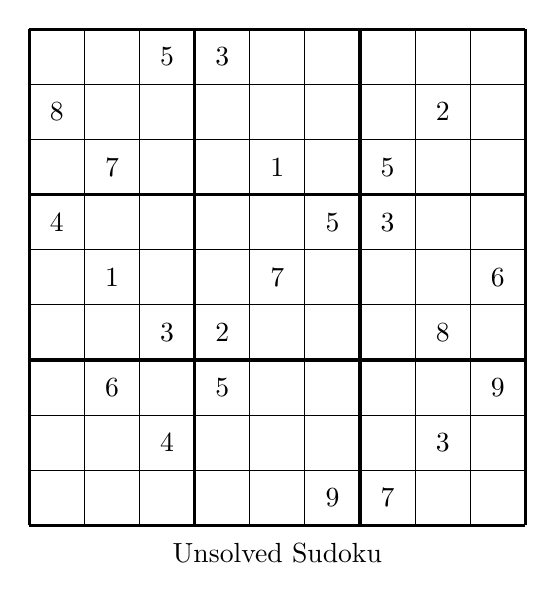
\begin{tikzpicture}[scale=.7]
  \begin{scope}
    \draw (0, 0) grid (9, 9);
    \draw[very thick, scale=3] (0, 0) grid (3, 3);

    \setcounter{row}{1}
    \setrow { }{ }{5}  {3}{ }{ }  { }{ }{ }
    \setrow {8}{ }{ }  { }{ }{ }  { }{2}{ }
    \setrow { }{7}{ }  { }{1}{ }  {5}{ }{ }

    \setrow {4}{ }{ }  { }{ }{5}  {3}{ }{ }
    \setrow { }{1}{ }  { }{7}{ }  { }{ }{6}
    \setrow { }{ }{3}  {2}{ }{ }  { }{8}{ }

    \setrow { }{6}{ }  {5}{ }{ }  { }{ }{9}
    \setrow { }{ }{4}  { }{ }{ }  { }{3}{ }
    \setrow { }{ }{ }  { }{ }{9}  {7}{ }{ }

    \node[anchor=center] at (4.5, -0.5) {Unsolved Sudoku};
  \end{scope}
\end{tikzpicture}
\end{center}

Numbers of each row must be unique, i.e., must contain all 9 numbers in range of 1..9 without repetition.
Same story for each column and also for each 3*3 square.

This puzzle is good candidate to try \ac{SMT} solver on, because it's essentially an unsolved system of equations.

\subsubsection{The first idea}

The only thing we must solve is that how to determine in one expression, if the input 9 variables has all 9 unique numbers?
They are not ordered or sorted, after all.

From the school-level mathematics, we can devise this idea:

\begin{equation}
\underbrace{10^{i_1} + 10^{i_2} + \cdots + 10^{i_9}}_9 = 1111111110
\end{equation}

Take each input variable, calculate $10^i$ and sum them all.
If all input values are unique, each will be settled at its own place.
Even more than that: there will be no holes, i.e., no skipped values.
So, in case of Sudoku, 1111111110 number will be final result, indicating that all 9 input variables are unique, in range of 1..9.

Exponentiation is heavy operation, can we use binary operations? Yes, just replace 10 with 2:

\begin{equation}
\underbrace{2^{i_1} + 2^{i_2} + \cdots + 2^{i_9}}_9 = 1111111110_2
\end{equation}

The effect is just the same, but the final value is in base 2 instead of 10.

Now a working example:

\lstinputlisting{SMT/sudoku_plus.py}

\begin{lstlisting}
\$ time python sudoku_plus.py
1 4 5 3 2 7 6 9 8
8 3 9 6 5 4 1 2 7
6 7 2 9 1 8 5 4 3
4 9 6 1 8 5 3 7 2
2 1 8 4 7 3 9 5 6
7 5 3 2 9 6 4 8 1
3 6 7 5 4 2 8 1 9
9 8 4 7 6 1 2 3 5
5 2 1 8 3 9 7 6 4

real    0m11.717s
user    0m10.896s
sys     0m0.068s
\end{lstlisting}

Even more, we can replace summing operation to logical OR:

\begin{equation}
\underbrace{2^{i_1} \vee 2^{i_2} \vee \cdots \vee 2^{i_9}}_9 = 1111111110_2
\end{equation}

% FIXME: только часть исходника + ссылка на github
\lstinputlisting{SMT/sudoku_or.py}

Now it works much faster. Z3 handles OR operation over bit vectors better than addition?

\begin{lstlisting}
\$ time python sudoku_or.py
1 4 5 3 2 7 6 9 8
8 3 9 6 5 4 1 2 7
6 7 2 9 1 8 5 4 3
4 9 6 1 8 5 3 7 2
2 1 8 4 7 3 9 5 6
7 5 3 2 9 6 4 8 1
3 6 7 5 4 2 8 1 9
9 8 4 7 6 1 2 3 5
5 2 1 8 3 9 7 6 4

real    0m1.429s
user    0m1.393s
sys     0m0.036s
\end{lstlisting}

The puzzle I used as example is dubbed as one of the hardest known
\footnote{\url{http://www.mirror.co.uk/news/weird-news/worlds-hardest-sudoku-can-you-242294}} (well, for humans).
It took ~1.4 seconds on my Intel Core i3-3110M 2.4GHz notebook to solve it. % FIXME tilde

\subsubsection{The second idea}

My first approach is far from effective, I did what first came to my mind and worked.
Another approach is to use \texttt{distinct} command from SMTLIB, which tells Z3 that some variables (of unspecific number) must be distinct (or unique).
This command is also available in Z3 Python interface.

I've rewritten my first Sudoku solver, now it operates over \textit{Int} \textit{sort}, it has \texttt{distinct} commands instead of bit operations,
and now also other constaint added: each cell value must be in 1..9 range, because, otherwise, Z3 will offer (although correct) solution with too big
and/or negative numbers.

% FIXME: только часть исходника + ссылка на github
\lstinputlisting{SMT/sudoku2.py}

\begin{lstlisting}
\$ time python sudoku2.py
1 4 5 3 2 7 6 9 8
8 3 9 6 5 4 1 2 7
6 7 2 9 1 8 5 4 3
4 9 6 1 8 5 3 7 2
2 1 8 4 7 3 9 5 6
7 5 3 2 9 6 4 8 1
3 6 7 5 4 2 8 1 9
9 8 4 7 6 1 2 3 5
5 2 1 8 3 9 7 6 4

real    0m0.382s
user    0m0.346s
sys     0m0.036s
\end{lstlisting}

That's much faster.

\subsubsection{Conclusion}

The awesomeness of \ac{SMT}-solvers is that our Sudoku solver has nothing else, we have just defined relationships between variables (cells).

\subsubsection{Homework}

As it seems, true Sudoku puzzle is the one which has only one solution.
The piece of code I've included in this article shows only the first one.
Using the method described earlier (\ref{SMTEnumerate}, also called ``model counting''), 
try to find more solutions, or prove that the solution you have just found is the only one possible.

\subsubsection{Further reading}

\url{http://www.norvig.com/sudoku.html}

\subsubsection{Sudoku as a \ac{SAT} problem}

It's also possible to represend Sudoku puzzle as a huge \ac{CNF} equation and use \ac{SAT}-solver to find solution, but it's just trickier.

Some articles about it\footnote{Another one: \url{http://ocw.mit.edu/courses/electrical-engineering-and-computer-science/6-005-elements-of-software-construction-fall-2011/assignments/MIT6_005F11_ps4.pdf}}: \cite{Sudoku1}, \cite{Sudoku2}, \cite{Sudoku3}.

\ac{SMT}-solver can also use \ac{SAT}-solver in its core, so it does all mundane translating work.
As a ``compiler'', it may not do this in the most efficient way, though.


\input{SMT/pe31.tex}
\subsection{Using Z3 theorem prover to prove equivalence of some weird alternative to XOR operation}

(The article was first published in my blog at April 2015: \url{http://blog.yurichev.com/node/86}).

There is a "A Hacker's Assistant" program\footnote{\url{http://www.hackersdelight.org/}} (\textit{Aha!}) written by Henry Warren,
who is also the author of the great "Hacker's Delight" book.

The \textit{Aha!} program is essentially \textit{superoptimizer}\footnote{\url{http://en.wikipedia.org/wiki/Superoptimization}},
which blindly brute-force a list of some generic RISC CPU instructions to achieve shortest possible (and jumpless or branch-free) 
CPU code sequence for desired operation.
For example, \textit{Aha!} can find jumpless version of abs() function easily.

Compiler developers use superoptimization to find shortest possible (and/or jumpless) code, but I tried to do otherwise -- to find longest code for some basic operation.
I tried \textit{Aha!} to find equivalent of basic XOR operation without usage of the actual XOR instruction, and the most bizarre example \textit{Aha!} gave is:

\begin{lstlisting}
Found a 4-operation program:
   add   r1,ry,rx
   and   r2,ry,rx
   mul   r3,r2,-2
   add   r4,r3,r1
   Expr: (((y & x)*-2) + (y + x))
\end{lstlisting}

And it's hard to say, why/where we can use it, maybe for obfuscation, I'm not sure.
I would call this \textit{suboptimization} (as opposed to \textit{superoptimization}). Or maybe \textit{superdeoptimization}.

But my another question was also, is it possible to prove that this is correct formula at all?
The \textit{Aha!} checking some intput/output values against XOR operation, but of course, not all the possible values.
It is 32-bit code, so it may take very long time to try all possible 32-bit inputs to test it.

We can try Z3 theorem prover for the job. It's called ``prover'', after all.

So I wrote this:

\begin{lstlisting}
#!/usr/bin/python
from z3 import *

x = BitVec('x', 32)
y = BitVec('y', 32)
output = BitVec('output', 32)
s = Solver()
s.add(x^y==output)
s.add(((y & x)*0xFFFFFFFE) + (y + x)!=output)
print s.check()
\end{lstlisting}

In plain English language, this means "are there any case for x and y where $x \oplus y$ doesn't equals to $((y \& x)*-2) + (y + x)$?"
... and Z3 prints "unsat", meaning, it can't find any counterexample to the equation.
So this \textit{Aha!} output is proved to be working just like XOR operation.

Oh, I also tried to extend the formula to 64-bit:

\begin{lstlisting}
#!/usr/bin/python
from z3 import *

x = BitVec('x', 64)
y = BitVec('y', 64)
output = BitVec('output', 64)
s = Solver()
s.add(x^y==output)
s.add(((y & x)*0xFFFFFFFE) + (y + x)!=output)
print s.check()
\end{lstlisting}

Nope, now it says "sat", meaning, Z3 found at least one counterexample.
Oops, it's because I forgot to extend -2 number to 64-bit value:

\begin{lstlisting}
#!/usr/bin/python
from z3 import *

x = BitVec('x', 64)
y = BitVec('y', 64)
output = BitVec('output', 64)
s = Solver()
s.add(x^y==output)
s.add(((y & x)*0xFFFFFFFFFFFFFFFE) + (y + x)!=output)
print s.check()
\end{lstlisting}

Now it says "unsat", so the formula given by \textit{Aha!} works for 64-bit code as well.

\subsubsection{In SMT-LIB form}

Now we can rephrase our equation to more suitable form: $(x + y - ((x \& y)<<1))$.
It also works well is Z3:

\begin{lstlisting}
#!/usr/bin/python
from z3 import *

x = BitVec('x', 64)
y = BitVec('y', 64)
output = BitVec('output', 64)
s = Solver()
s.add(x^y==output)
s.add((x + y - ((x & y)<<1)) != output)
print s.check()
\end{lstlisting}

Here is how to define it in SMT-LIB way:

\begin{lstlisting}
(declare-const x (_ BitVec 64))
(declare-const y (_ BitVec 64))
(assert 
	(not
		(=
			(bvsub
				(bvadd x y)
				(bvshl (bvand x y) (_ bv1 64)))
			(bvxor x y)
		)
	)
)
(check-sat)
\end{lstlisting}

\subsubsection{Using universal quantifier}

Z3 has universal quantifier \TT{exists}, which defines a constraint, which is true if at least one set of variables satistfied underlying condition:

\begin{lstlisting}
(declare-const x (_ BitVec 64))
(declare-const y (_ BitVec 64))
(assert 
	(exists ((x (_ BitVec 64)) (y (_ BitVec 64)))
		(not (=
			(bvsub 
				(bvadd x y)
				(bvshl (bvand x y) (_ bv1 64))
			)
			(bvxor x y)
		))
	)
)
(check-sat)
\end{lstlisting}

It returns ``unsat'', meaning, Z3 couldn't find any counterexample of the equation, i.e., it's not exist.\\
\\
This is also known as $\exists$ in mathematical logic lingo.\\
\\
Z3 has also universal quantifier \TT{forall}, which defines a constraint, where all possible values for the equation must be true.
So we can rewrite our \ac{SMT} example as:

\begin{lstlisting}
(declare-const x (_ BitVec 64))
(declare-const y (_ BitVec 64))
(assert 
	(forall ((x (_ BitVec 64)) (y (_ BitVec 64)))
		(=
			(bvsub 
				(bvadd x y)
				(bvshl (bvand x y) (_ bv1 64))
			)
			(bvxor x y)
		)
	)
)
(check-sat)
\end{lstlisting}

It returns \TT{sat}, meaning, the equation is correct for all possible 64-bit \TT{x} and \TT{y} values, like them all were checked.

Mathematically speaking: $\forall n\!\in\!\mathbb{N}\; (x \oplus y = (x + y - ((x \& y)<<1)))$
\footnote{
$\forall$ means \textit{equation must be true for all possible values}, which are choosen from natural numbers ($\mathbb{N}$).}

\subsubsection{How the equation works}

First of all, binary addition can be viewed as binary XORing with carrying (\ref{adder}).
Here is an example: let's add 2 (10b) and 2 (10b).
XORing these two values resulting 0, but there is a carry generated during addition of two second bits.
That carry bit is propagated further and settles at the place of the 3rd bit: 100b.
4 (100b) is hence a final result of addition.

If the carry bits are not generated during addition, the addition operation is merely XORing.
For example, let's add 1 (1b) and 2 (10b). $1 + 2$ equals to 3, but $1 \oplus 2$ is also 3.

If the addition is XORing plus carry generation and application, we should eliminate effect of carrying somehow here.
The first part of the equation ($x + y$) is addition, the second ($(x \& y)<<1$) is just calculation of every carry bit which was used during addition.
Subtracting removes carry bits from the result of addition, so the only XOR effect is left then.

It's hard to say how Z3 proves this: maybe it just simplifies the equation down to single XOR using simple boolean algebra rewriting rules?

   % \\
\input{SMT/Dietz.tex} % //
% FIXME \ac{}
\subsection{Cracking LCG with Z3 SMT solver}

% FIXME first appeared in blog...

There are well-known weaknesses of LCG (
\href{http://en.wikipedia.org/wiki/Linear_congruential_generator#Advantages_and_disadvantages_of_LCGs}{1},
\href{http://www.reteam.org/papers/e59.pdf}{2}, % FIXME \cite
\href{http://stackoverflow.com/questions/8569113/why-1103515245-is-used-in-rand/8574774#8574774}{3}
), but let's see, if it would be possible to crack it straightforwardly, without any special knowledge.
We would define all relations between LCG states in term of Z3 SMT solver.
(I first made attempt to do it using \href{https://reference.wolfram.com/language/ref/FindInstance.html}{FindInstance} in Wolfram Mathematica, but failed, perhaps, made a mistake somewhere).
Here is a test progam:

\begin{lstlisting}
#include <stdlib.h>
#include <stdio.h>
#include <time.h>

int main()
{
	int i;

	srand(time(NULL));

	for (i=0; i<10; i++)
		printf ("%d\n", rand()%100);
};
\end{lstlisting}

It is intended to print 10 pseudorandom numbers in 0..99 range.
So it does:

\begin{lstlisting}
37
29
74
95
98
40
23
58
61
17
\end{lstlisting}

Let's say we are observing only 8 of these numbers (from 29 to 61) and we need to predict next one (17) and/or previous one (37).

The program is compiled using MSVC 2013 (I choose it because its LCG is simpler than that in Glib):

\begin{lstlisting}
.text:0040112E rand            proc near
.text:0040112E                 call    __getptd
.text:00401133                 imul    ecx, [eax+0x14], 214013
.text:0040113A                 add     ecx, 2531011
.text:00401140                 mov     [eax+14h], ecx
.text:00401143                 shr     ecx, 16
.text:00401146                 and     ecx, 7FFFh
.text:0040114C                 mov     eax, ecx
.text:0040114E                 retn
.text:0040114E rand            endp
\end{lstlisting}

This is very simple LCG, but the result is not clipped state, but it's rather shifted by 16 bits.
Let's define LCG in Z3:

\begin{lstlisting}
#!/usr/bin/python
from z3 import *

output_prev = BitVec('output_prev', 32)
state1 = BitVec('state1', 32)
state2 = BitVec('state2', 32)
state3 = BitVec('state3', 32)
state4 = BitVec('state4', 32)
state5 = BitVec('state5', 32)
state6 = BitVec('state6', 32)
state7 = BitVec('state7', 32)
state8 = BitVec('state8', 32)
state9 = BitVec('state9', 32)
state10 = BitVec('state10', 32)
output_next = BitVec('output_next', 32)

s = Solver()

s.add(state2 == state1*214013+2531011)
s.add(state3 == state2*214013+2531011)
s.add(state4 == state3*214013+2531011)
s.add(state5 == state4*214013+2531011)
s.add(state6 == state5*214013+2531011)
s.add(state7 == state6*214013+2531011)
s.add(state8 == state7*214013+2531011)
s.add(state9 == state8*214013+2531011)
s.add(state10 == state9*214013+2531011)

s.add(output_prev==URem((state1>>16)&0x7FFF,100))
s.add(URem((state2>>16)&0x7FFF,100)==29)
s.add(URem((state3>>16)&0x7FFF,100)==74)
s.add(URem((state4>>16)&0x7FFF,100)==95)
s.add(URem((state5>>16)&0x7FFF,100)==98)
s.add(URem((state6>>16)&0x7FFF,100)==40)
s.add(URem((state7>>16)&0x7FFF,100)==23)
s.add(URem((state8>>16)&0x7FFF,100)==58)
s.add(URem((state9>>16)&0x7FFF,100)==61)
s.add(output_next==URem((state10>>16)&0x7FFF,100))

print(s.check())
print(s.model())
\end{lstlisting}

URem states for \textit{unsigned remainder}.
It works for some time and gave us correct result!

\begin{lstlisting}
sat
[state3 = 2276903645,
 state4 = 1467740716,
 state5 = 3163191359,
 state7 = 4108542129,
 state8 = 2839445680,
 state2 = 998088354,
 state6 = 4214551046,
 state1 = 1791599627,
 state9 = 548002995,
 output_next = 17,
 output_prev = 37,
 state10 = 1390515370]
\end{lstlisting}

% FIXME tilde
I added ~10 states to be sure result will be correct. It may be not if you supply lesser amount of PRNG numbers.

That is the reason why LCG is not suitable for any security-related task.
This is why \href{https://en.wikipedia.org/wiki/Cryptographically_secure_pseudorandom_number_generator}{cryptographically secure pseudorandom number generators} are exist: they are designed to be protected against such simple attack.
Well, at least if \href{https://en.wikipedia.org/wiki/Dual_EC_DRBG}{NSA is not involved}.

As far, as I can understand, \href{http://en.wikipedia.org/wiki/Security_token}{security tokens} like \href{http://en.wikipedia.org/wiki/RSA_SecurID}{RSA SecurID} can be viewed just as \ac{CPRNG} with a secret seed.
It shows new pseudorandom number each minute, and the server can predict it, because it knows the seed.
Imagine if such token would implement LCG -- it would be much easier to break!


\section{KLEE}

% subsections:
\subsection{School-level equation}

Let's revisit school-level system of equations from (\ref{eq2_SMT}).

We will force KLEE to find a path, where all the constraints are satisfied:

\lstinputlisting{KLEE/klee_eq1.c}

% FIXME:
\begin{lstlisting}
\$ clang -emit-llvm -c -g klee_eq.c
...

\$ klee klee_eq.bc
KLEE: output directory is "/home/klee/klee-out-93"
KLEE: WARNING: undefined reference to function: klee_assert
KLEE: WARNING ONCE: calling external: klee_assert(0)
KLEE: ERROR: /home/klee/klee_eq.c:18: failed external call: klee_assert
KLEE: NOTE: now ignoring this error at this location

KLEE: done: total instructions = 32
KLEE: done: completed paths = 1
KLEE: done: generated tests = 1
\end{lstlisting}

Let's find out, where \TT{klee\_assert()} has been triggered:

% FIXME:
\begin{lstlisting}
\$ ls klee-last | grep err
test000001.external.err

\$ ktest-tool --write-ints klee-last/test000001.ktest
ktest file : 'klee-last/test000001.ktest'
args       : ['klee_eq.bc']
num objects: 3
object    0: name: b'circle'
object    0: size: 4
object    0: data: 5
object    1: name: b'square'
object    1: size: 4
object    1: data: 2
object    2: name: b'triangle'
object    2: size: 4
object    2: data: 1
\end{lstlisting}

This is indeed correct solution to the system of equations.

KLEE has intrinsic \TT{klee\_assume()} which tells KLEE to cut path if some constraint is not true.
So we can rewrite our example in such cleaner way:

\lstinputlisting{KLEE/klee_eq2.c}



\subsection{Zebra puzzle (\ac{AKA} Einstein puzzle)}
\label{zebra_SMT}

Zebra puzzle is a popular puzzle, defined as follows:

% FIXME remove paragraph at first line
\begin{framed}
\begin{quotation}
1.There are five houses.\\
2.The Englishman lives in the red house.\\
3.The Spaniard owns the dog.\\
4.Coffee is drunk in the green house.\\
5.The Ukrainian drinks tea.\\
6.The green house is immediately to the right of the ivory house.\\
7.The Old Gold smoker owns snails.\\
8.Kools are smoked in the yellow house.\\
9.Milk is drunk in the middle house.\\
10.The Norwegian lives in the first house.\\
11.The man who smokes Chesterfields lives in the house next to the man with the fox.\\
12.Kools are smoked in the house next to the house where the horse is kept.\\
13.The Lucky Strike smoker drinks orange juice.\\
14.The Japanese smokes Parliaments.\\
15.The Norwegian lives next to the blue house.\\
\\
Now, who drinks water? Who owns the zebra?\\
\\
In the interest of clarity, it must be added that each of the five houses is painted a different color, and their inhabitants are of different national extractions, own different pets, drink different beverages and smoke different brands of American cigarets [sic]. One other thing: in statement 6, right means your right.
\end{quotation}
\end{framed}
( \url{https://en.wikipedia.org/wiki/Zebra_Puzzle} ) \\
\\
It's a very good example of constraint satisfaction problem (CSP). % FIXME \ac

We would encode each entity as integer variable, representing number of house.

Then, to define that Englishman lives in red house, we will define this constraint: \TT{Englishman == Red}, meaning that number of a house where Englishmen resides and where tea is drunk is the same.

To define that Norwegian lives next to the blue house, we don't realy know, if it is at left side of blue house or at right side, but we know that house numbers are different by just 1.
So we will define this constraint: \TT{Norwegian==Blue-1 OR Norwegian==Blue+1}.

We will also need to limit all house numbers, so they will be in range of 1..5.

We will also use \TT{Distinct} to show that all various entities of the same type are all has different house numbers.

\lstinputlisting{SMT/zebra.py}

When we run it, we got correct result:

\begin{lstlisting}
sat
[Snails = 3,
 Blue = 2,
 Ivory = 4,
 OrangeJuice = 4,
 Parliament = 5,
 Yellow = 1,
 Fox = 1,
 Zebra = 5,
 Horse = 2,
 Dog = 4,
 Tea = 2,
 Water = 1,
 Chesterfield = 2,
 Red = 3,
 Japanese = 5,
 LuckyStrike = 4,
 Norwegian = 1,
 Milk = 3,
 Kools = 1,
 OldGold = 3,
 Ukrainian = 2,
 Coffee = 5,
 Green = 5,
 Spaniard = 4,
 Englishman = 3]
 \end{lstlisting}


\subsection{Sudoku}

I've also rewritten Sudoku example (\ref{sudoku_SMT}) for KLEE:

\lstinputlisting[numbers=left]{KLEE/klee_sudoku_or1.c}

Let's run it:

% FIXME:
\begin{lstlisting}
\$ clang -emit-llvm -c -g klee_sudoku_or1.c
...

\$ time klee klee_sudoku_or1.bc
KLEE: output directory is "/home/klee/klee-out-98"
KLEE: WARNING: undefined reference to function: klee_assert
KLEE: WARNING ONCE: calling external: klee_assert(0)
KLEE: ERROR: /home/klee/klee_sudoku_or1.c:93: failed external call: klee_assert
KLEE: NOTE: now ignoring this error at this location

KLEE: done: total instructions = 7512
KLEE: done: completed paths = 161
KLEE: done: generated tests = 161

real    3m44.111s
user    3m43.319s
sys     0m0.951s
\end{lstlisting}

Now this is really slower (on my Intel Core i3-3110M 2.4GHz notebook) in comparison to Z3Py solution (\ref{sudoku_SMT}).

But the answer is correct:

% FIXME:
\begin{lstlisting}
\$ ls klee-last | grep err
test000161.external.err

\$ ktest-tool --write-ints klee-last/test000161.ktest
ktest file : 'klee-last/test000161.ktest'
args       : ['klee_sudoku_or1.bc']
num objects: 1
object    0: name: b'cells'
object    0: size: 81
object    0: data: b'\x01\x04\x05\x03\x02\x07\x06\t\x08\x08\x03\t\x06\x05\x04\x01\x02\x07\x06\x07\x02\t\x01\x08\x05\x04\x03\x04\t\x06\x01\x08\x05\x03\x07\x02\x02\x01\x08\x04\x07\x03\t\x05\x06\x07\x05\x03\x02\t\x06\x04\x08\x01\x03\x06\x07\x05\x04\x02\x08\x01\t\t\x08\x04\x07\x06\x01\x02\x03\x05\x05\x02\x01\x08\x03\t\x07\x06\x04'
\end{lstlisting}

% FIXME backslash
\TT{\\t} is character with ASCII code of 9 in C/C++, and KLEE attempts to treat byte array as C/C++ string, so it shows some values in such way.
We can just remember that there is 9 at the each place where we see \TT{\\t}.
The solution, while not properly formatted, correct indeed. \\
\\
By the way, at lines 42, 43 you may see how we tell to KLEE that all array elements must be within some limits.
If we comment these lines out, we've got this:

% FIXME:
\begin{lstlisting}
\$ time klee klee_sudoku_or1.bc
KLEE: output directory is "/home/klee/klee-out-100"
KLEE: WARNING: undefined reference to function: klee_assert
KLEE: ERROR: /home/klee/klee_sudoku_or1.c:51: overshift error
KLEE: NOTE: now ignoring this error at this location
KLEE: ERROR: /home/klee/klee_sudoku_or1.c:51: overshift error
KLEE: NOTE: now ignoring this error at this location
KLEE: ERROR: /home/klee/klee_sudoku_or1.c:51: overshift error
KLEE: NOTE: now ignoring this error at this location
...
\end{lstlisting}

KLEE warns us that shift value at line 51 is too big.
Indeed, KLEE may try all byte values up to 255 (0xFF), which are pointless to use there, and may indicate error or bug, so KLEE warns about it.\\
\\
Now let's use \TT{klee\_assume()} again:

\lstinputlisting{KLEE/klee_sudoku_or2.c}

% FIXME:
\begin{lstlisting}
\$ time klee klee_sudoku_or2.bc
KLEE: output directory is "/home/klee/klee-out-99"
KLEE: WARNING: undefined reference to function: klee_assert
KLEE: WARNING ONCE: calling external: klee_assert(0)
KLEE: ERROR: /home/klee/klee_sudoku_or2.c:93: failed external call: klee_assert
KLEE: NOTE: now ignoring this error at this location

KLEE: done: total instructions = 7119
KLEE: done: completed paths = 1
KLEE: done: generated tests = 1

real    0m35.312s
user    0m34.945s
sys     0m0.318s
\end{lstlisting}

That works much faster: perhaps KLEE indeed handle this intrinsic in a special way.
And, as we see, the only one path is generated (one we actually interesting in it) instead of 161.

It's still much slower than Z3Py solution, though.


\input{KLEE/UNIXdatetime.tex}
\input{KLEE/base64.tex}
\subsection{CRC} % FIXME full name

\subsubsection{Buffer alteration case \#1}

Sometimes, you need to alter a piece of data which is \textit{protected} by some kind of checksum or \ac{CRC}, and you can't change checksum or CRC value, but can alter piece of data so that checksum will remain the same.

Let's pretend, we've got a piece of data with ``Hello, world!'' string at the beginning and ``and goodbye'' string at the end.
We can alter 14 characters at the middle, but for some reason, they must be in \textit{a..z} limits, but we can put any characters there.
CRC64 of the whole block must be \TT{0x12345678abcdef12}.

Let's see\footnote{There are several slightly different CRC64 implementations, the one I use here can also be different from popular ones.}:

\lstinputlisting{KLEE/klee_CRC64.c}

Since our code uses memcmp() standard C/C++ function, we need to add \TT{--libc=uclibc} switch, so KLEE will use its own uClibc % FIXME check spelling
implementation. % \ref{} -> closed programs

% FIXME:
\begin{lstlisting}
\$ clang -emit-llvm -c -g klee_CRC64.c

\$ time klee --libc=uclibc klee_CRC64.bc
\end{lstlisting}

It takes about 1 minute (on my XXX) and we getting this:

% FIXME:
\begin{lstlisting}
...
real    0m52.643s
user    0m51.232s
sys     0m0.239s
...
\$ ls klee-last | grep err
test000001.user.err
test000002.user.err
test000003.user.err
test000004.external.err

\$ ktest-tool --write-ints klee-last/test000004.ktest
ktest file : 'klee-last/test000004.ktest'
args       : ['klee_CRC64.bc']
num objects: 1
object    0: name: b'buf'
object    0: size: 46
object    0: data: b'Hello, world!.. qqlicayzceamyw ... and goodbye'
\end{lstlisting}

Maybe it's slow, but definitely faster than bruteforce.
Indeed, $log_2{26^{14}} \approx 65.8$
which is close to 64 bits.
In other words, one need $\approx 14$ latin characters to encode 64 bits.
And KLEE + \ac{SMT} solver needs 64 bits at some place it can alter to make final CRC64 value equal to what we defined.

I tried to reduce length of the \textit{middle block} to 13 characters: no luck for KLEE then, it has no space enough.

\subsubsection{Buffer alteration case \#2}

I went sadistic: what if the buffer must contain the CRC64 value which, after calculation of CRC64, will result in the same value?
Fascinately, % FIXME check spelling
KLEE can solve this.
The buffer will have the following format:

% FIXME:
\begin{lstlisting}
Hello, world! <8-bytes (64-bit value)> and goodbye <6 more bytes>
\end{lstlisting}

% FIXME:
\begin{lstlisting}
int main()
{
#define HEAD_STR "Hello, world!.. "
#define HEAD_SIZE strlen(HEAD_STR)
#define TAIL_STR " ... and goodbye"
#define TAIL_SIZE strlen(TAIL_STR)
// 8 bytes for 64-bit value:
#define MID_SIZE 8
#define BUF_SIZE HEAD_SIZE+TAIL_SIZE+MID_SIZE+6

	char buf[BUF_SIZE];
  
	klee_make_symbolic(buf, sizeof buf, "buf");

	klee_assume (memcmp (buf, HEAD_STR, HEAD_SIZE)==0);

	klee_assume (memcmp (buf+HEAD_SIZE+MID_SIZE, TAIL_STR, TAIL_SIZE)==0);
	
	uint64_t mid_value=*(uint64_t*)(buf+HEAD_SIZE);
	klee_assume (crc64 (0, buf, BUF_SIZE)==mid_value);

	klee_assert(0);

	return 0;
}
\end{lstlisting}

It works:

% FIXME:
\begin{lstlisting}
\$ time klee --libc=uclibc klee_CRC64.bc
...
real    5m17.081s
user    5m17.014s
sys     0m0.319s

\$ ls klee-last | grep err
test000001.user.err
test000002.user.err
test000003.external.err

\$ ktest-tool --write-ints klee-last/test000003.ktest
ktest file : 'klee-last/test000003.ktest'
args       : ['klee_CRC64.bc']
num objects: 1
object    0: name: b'buf'
object    0: size: 46
object    0: data: b'Hello, world!.. T+]\xb9A\x08\x0fq ... and goodbye\xb6\x8f\x9c\xd8\xc5\x00'
\end{lstlisting}

8 bytes between two strings is 64-bit value which equals to CRC64 of this whole block.
Again, it's faster than brute-force way to find it.
If to decrease last spare 6-byte buffer to 4 bytes or less, KLEE works so long so I've stopped it.

\subsubsection{Recovering input data for given CRC32 value of it}

I've always wanted to do so, but everyone knows this is impossible for input buffers larger than 4 bytes.
As my experiments show, it's still possible for tiny input buffers of data, constrained in some way.

The CRC32 value of 6-byte ``SILVER'' string is known: \TT{0xDFA3DFDD}.
KLEE can find this 6-byte string, if it knows that each byte of input buffer is in \textit{A..Z} limits:

\lstinputlisting[numbers=left]{KLEE/klee_SILVER.c}

% FIXME:
\begin{lstlisting}
\$ clang -emit-llvm -c -g klee_SILVER.c
...

\$ klee klee_SILVER.bc
...

\$ ls klee-last | grep err
test000013.external.err

\$ ktest-tool --write-ints klee-last/test000013.ktest
ktest file : 'klee-last/test000013.ktest'
args       : ['klee_SILVER.bc']
num objects: 1
object    0: name: b'str'
object    0: size: 6
object    0: data: b'SILVER'
\end{lstlisting}

Still, it's no magic: if to remove condition at lines 23..25 (i.e., if to relax constraints),
KLEE will produce some other string, which will be still correct for the CRC32 value given.

It works, because 6 Latin characters in \textit{A..Z} limits contain $\approx 28.2$ bits:
$log_2{26^6} \approx 28.2$, which is even smaller value than 32.
In other words, the final CRC32 value holds enough bits to recover $\approx 28.2$ bits of input.

The input buffer can be even bigger, if each byte of it will be in even tighter % FIXME spelling
constraints (decimal digits, binary digits, etc).

\subsubsection{In comparison with other hashing algorithms}

Things are that easy for some other hashing algorithms like \textit{fletcher checksum}, % FIXME URL
but not for cryptographically secure ones (like MD5, SHA1, etc), they are protected from such simple cryptoanalysis. % FIXME \ref{} -> am.crypto


\input{KLEE/LZSS.tex}

\subsection{Exercise}

Here is my crackme/keygenme, which may be tricky, but easy to solve using KLEE:
\url{http://challenges.re/74/}.



\input{SMT/rockey.tex}

